\subsection{Path Following}
\label{sec:pathfollowing}
We want the movement of units to appear at least somewhat smooth rather than having them jerk from cell to cell. Additionally, we do not want units to simply pass through one another, so some form of collision avoidance is required. Both of these problems can be solved by steering behaviour found in flocking. The primary aspects of flocking we will be using are seeking behaviour and fleeing behaviour. We will also explore the problems that occur when applying these techniques on paths.

\subsubsection{Steering}
In steering behaviours, all characters have a vector indicating their movement. These vectors are influenced through steering, which is applying other vectors to this vector, possibly making use of the current movement. When applying these vectors, we take into account a mass for the character being moved, as well as a maximum force (steering vector length) that can be applied and a maximum speed. We will use fleeing and seeking behaviour only. The resulting steering vector is the sum of all seeking and fleeing vectors that apply to a character, all scaled with a weight. In the case that the result exceeds the maximum force, it is scaled to that maximum. The steering force and old movement vector are then put in a weighted sum, which is then cropped to the maximum speed to form the new movement vector. Since steering calculations are done very frequently, we use optimized code, such as seen in section \ref{sec:euclidean}.

\subsubsection{Seeking}
Seeking is usually used on a single point per character, as they can only move to one point at a time. Since the primary task is to get somewhere, the vector from seeking gets added in after combining and scaling the other vectors, so it has a set primary part in the movement. Desired seeking force is simply determined by subtracting the position of the seeking character from that of the seeking point: $DesiredSeekingForce = SeekingPosition - CharacterPosition$. Of course, this force has to be in similar realms as the current movement, so it gets scaled to the same length as that.

\paragraph{Arrival}
Arrival is applied after the seeking vector is determined. Once we are close enough to the target, we want to slow down. We have to give a certain arrival radius in which the arrival behaviour starts to take place. Once in the arrival radius, we calculate the factor with which we will scale the seeking vector. The factor is determined as follows: $Factor = \frac{DistanceFromTarget}{ArrivalRadius}$.

\subsubsection{Fleeing}
Fleeing works similarly to arriving, but in the opposite direction and is weighted less, as it is secondary movement. First the fleeing radius is checked, and if the distance between the fleeing point and the character is smaller than this radius, we simply ignore fleeing from this point. The vector we use for our direction is the same as the one for seeking force, but multiplied by $-1$ to go in the other direction: $DesiredFleeingForce = CharaterPosition - FleeingPosition$. This vector, again, must be scaled to have the same length as the old movement vector. Within the radius, we have to check what the distance is from the edge of the radius, rather the fleeing point. This distance becomes a similar factor to the one in arrival: $Factor = \frac{DistanceFromEdge}{ArrivalRadius}$. With this factor, we scale our fleeing force, and we have our final fleeing force from one point.

\subsubsection{Solid Cells}
\label{sec:solid_cells}
We originally intended to simply have bounding squares around solid cells. These would make sure that any movement vector going into them gets cropped. Due to the way we ended up handling refresh rate inconsistency in the game, this was sadly not an option within this part of the software. We scaled the vector with the time difference in between ticks, so cutting a vector short would not properly fix the problem.

Instead, we just applied fleeing behaviour towards the solid cells. The weight of the fleeing vector for this purpose would far exceed that of the other steering vectors. The problem with this is that fleeing uses circular fleeing areas, so the walls would be bumpy in effect, and allow characters to pass in between them at times. We fixed this by instead using Chebyshev distance as seen in section \ref{sec:chebyshev}, for purposes of the fleeing radius and the scaling calculations for the fleeing vector. The square shape allows us to keep walls nice and smooth. Additionally, we add extra weight to the greater force among the horizontal and vertical force. This way characters are more pushed out of a wall than pushed back.

\subsubsection{Group Arrival}
Group arrival will be done slightly differently from the arrival of singular units. First of all, when a group of units get to their goal, they do not adjust to the exact position. Instead of adjusting or trying to get into once cell together, they all flock to the center of the cell until they are within a radius from it, based on the group size. 

\subsubsection{The Scooping Problem}
\begin{wrapfigure}{r}{0.30\textwidth}
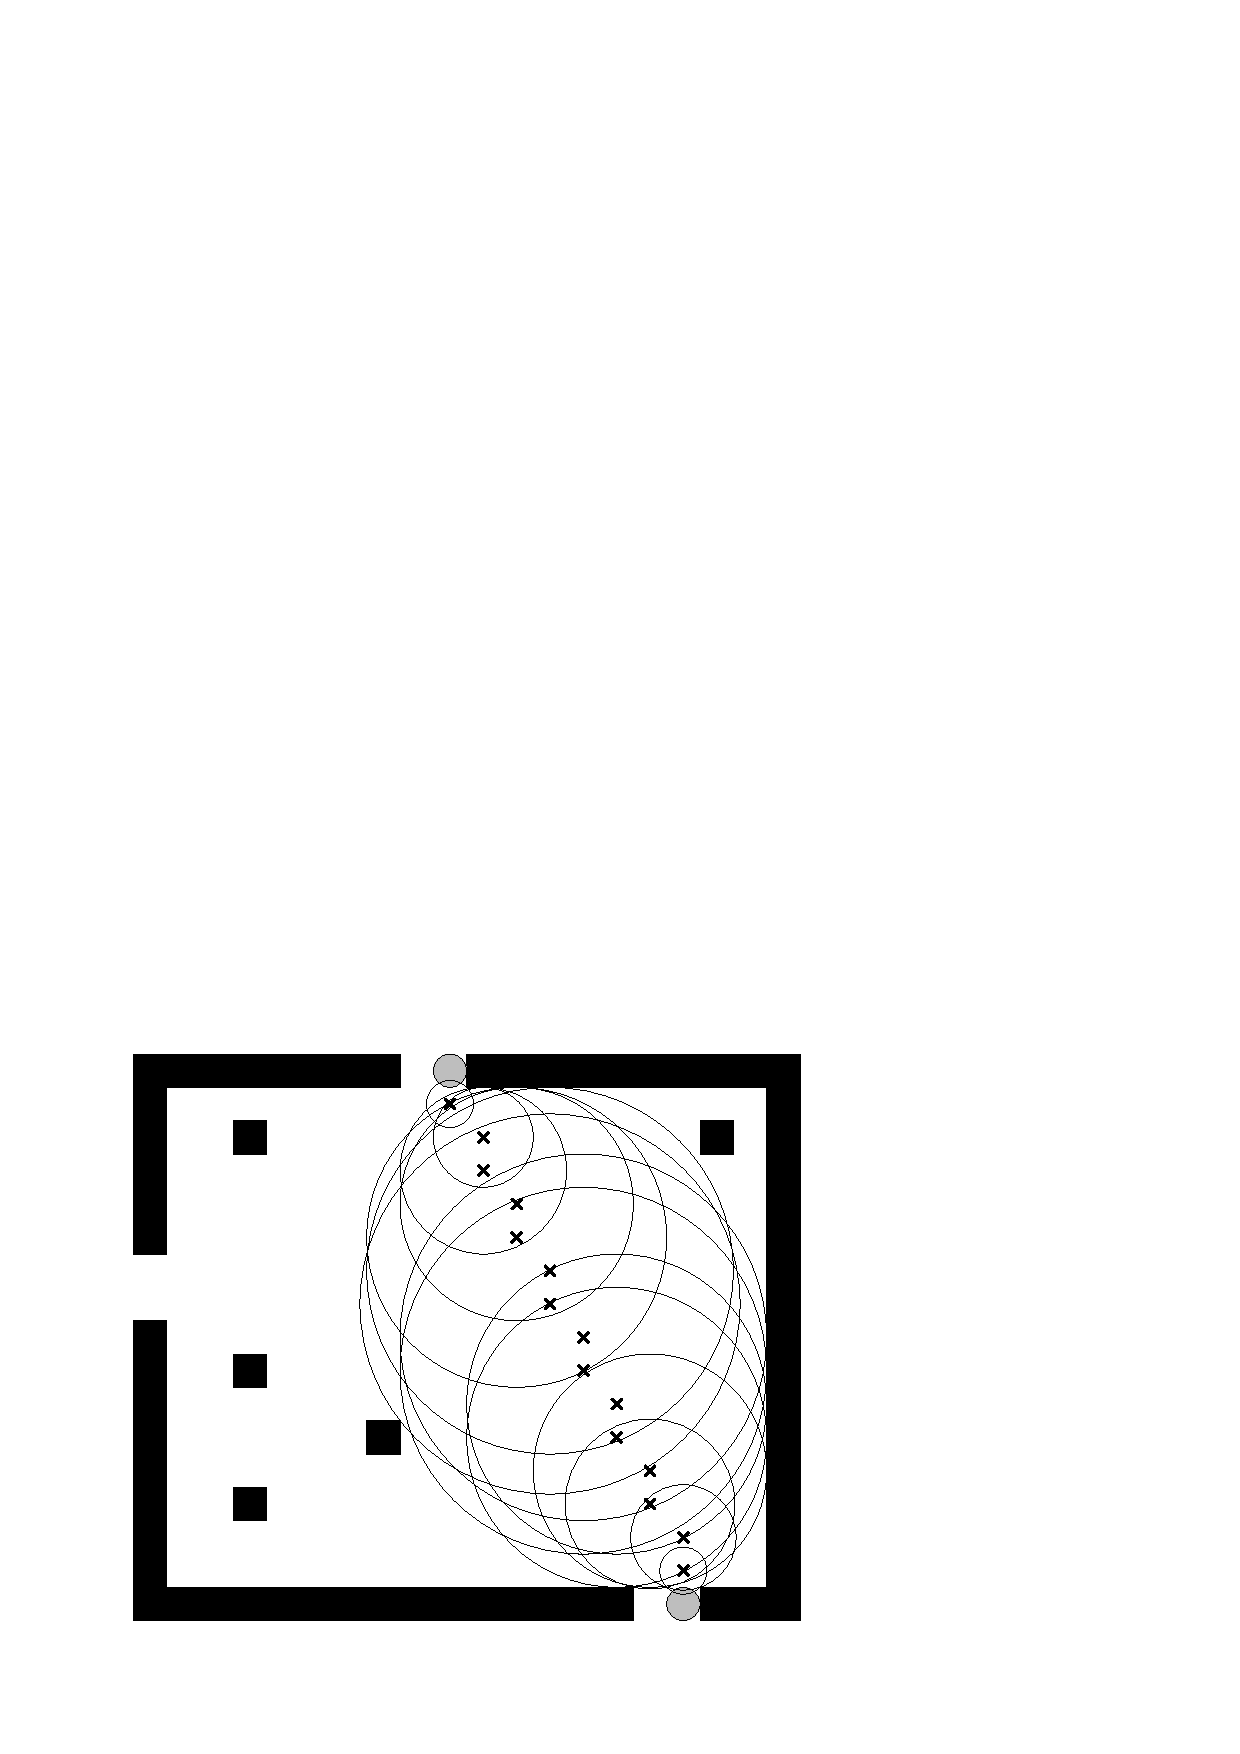
\includegraphics[width=0.30\textwidth]{images/clear_path1.pdf}
\caption{A clear and open path}
\label{fig:clear_path}
\end{wrapfigure} 
\begin{wrapfigure}{r}{0.30\textwidth}
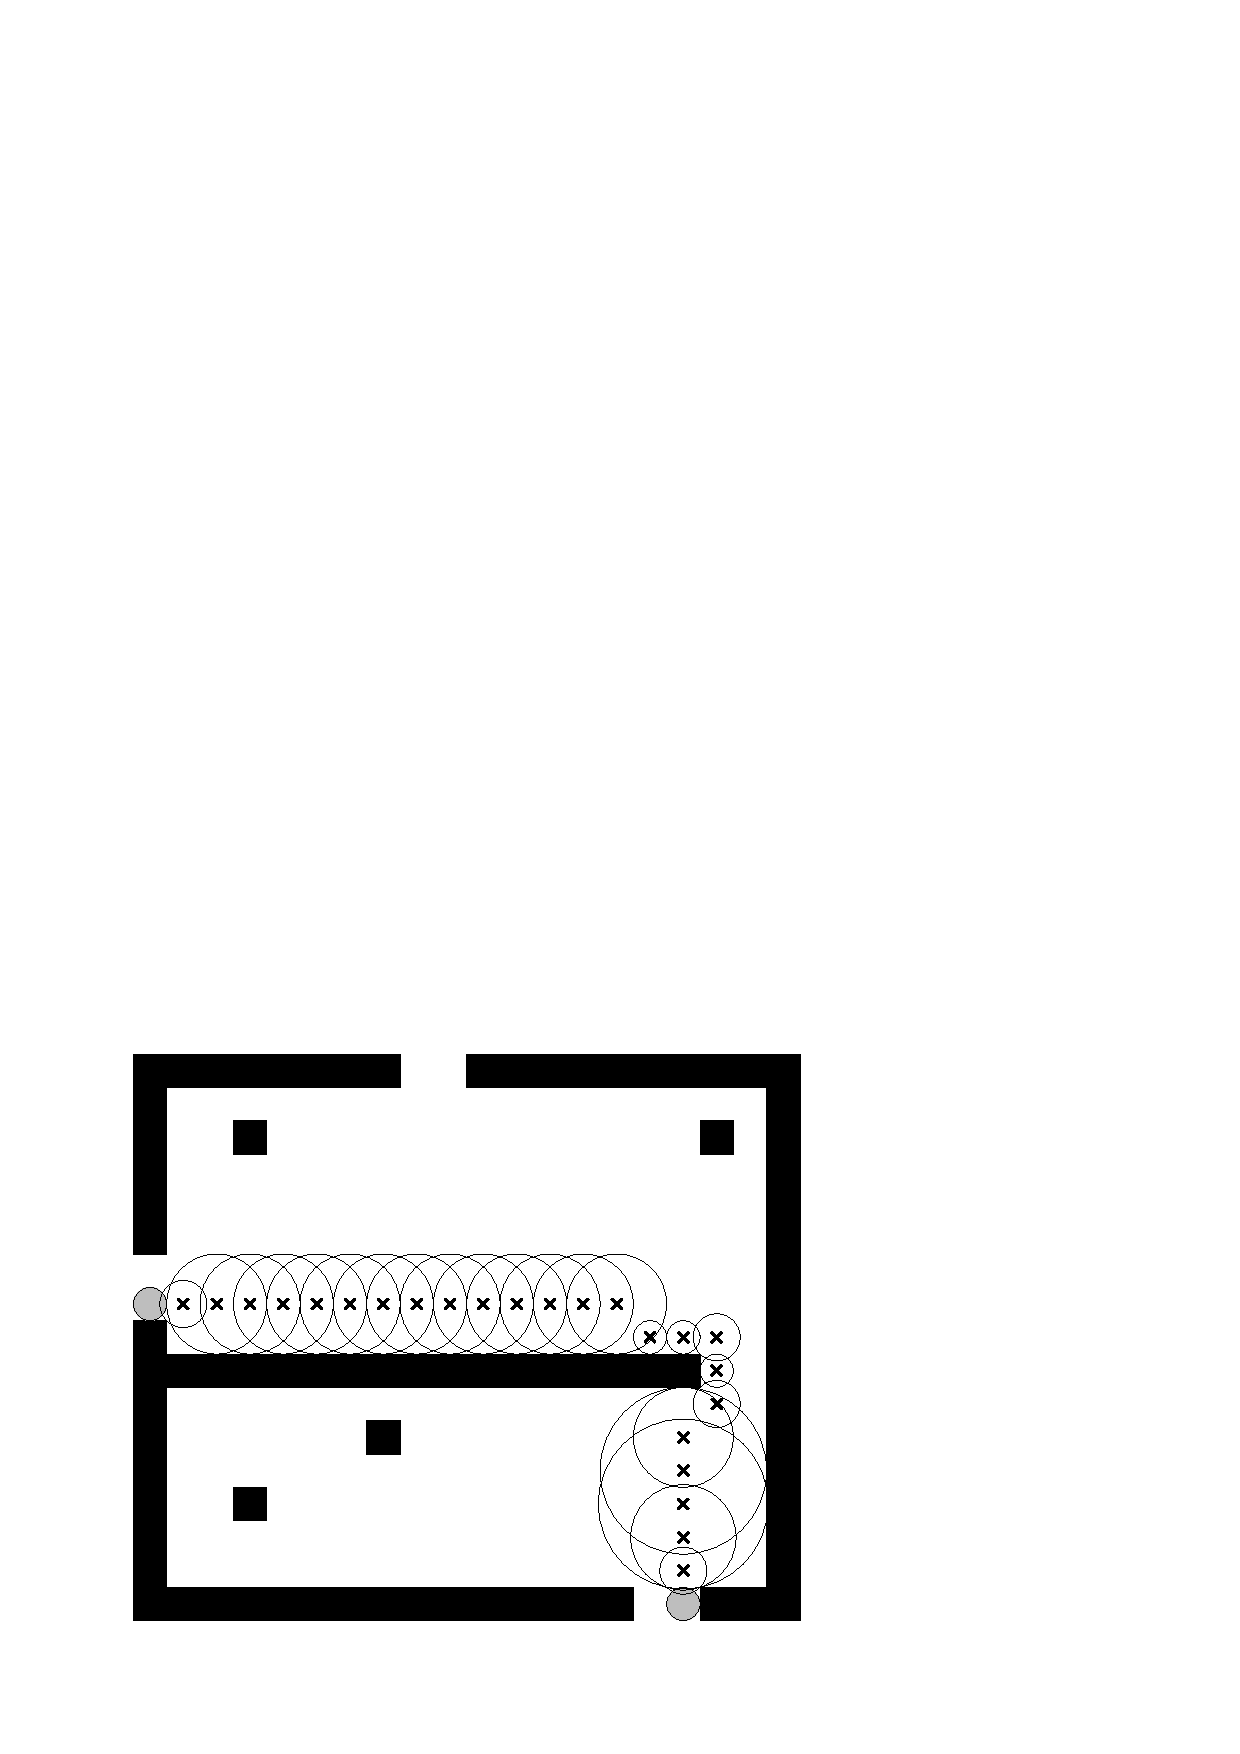
\includegraphics[width=0.30\textwidth]{images/scoop_path1.pdf}
\caption{The scooping problem}
\label{fig:scoop_path}
\end{wrapfigure} 
Since flocking allows groups to move together, we do not want to force all members of a group to first get into a cell before moving to the next one. Instead, we just let them flock to within a radius of the target cell, its travel radius, then they move on to the next. This creates a problem when a group encounters the start of a wall. The units have to walk on one side of the wall to reach their final destination. The wall may scoop some of the group to the other side, because it is still within travel radius of their target cell.

In order to fix this problem, determine the radii of the cells upon creation or loading of the map. These radii will be the distance from the center of the cell to the edge of the closest static obstacle. This allows groups to move very freely towards their goal in open fields, while making sure they correctly funnel into finer areas. Figure \ref{fig:clear_path} shows the freedom characters would have when steering along a path in an open area. Figure \ref{fig:scoop_path} shows how the movements of characters becomes more regulated when a case of the scooping problem occurs. Characters have to move along the end of the wall before they may consider the cells on the other side of the wall their targets.

\subsubsection{Wall Hugging Slowdown}
\label{sec:extra_weight}
\begin{wrapfigure}{r}{0.30\textwidth}
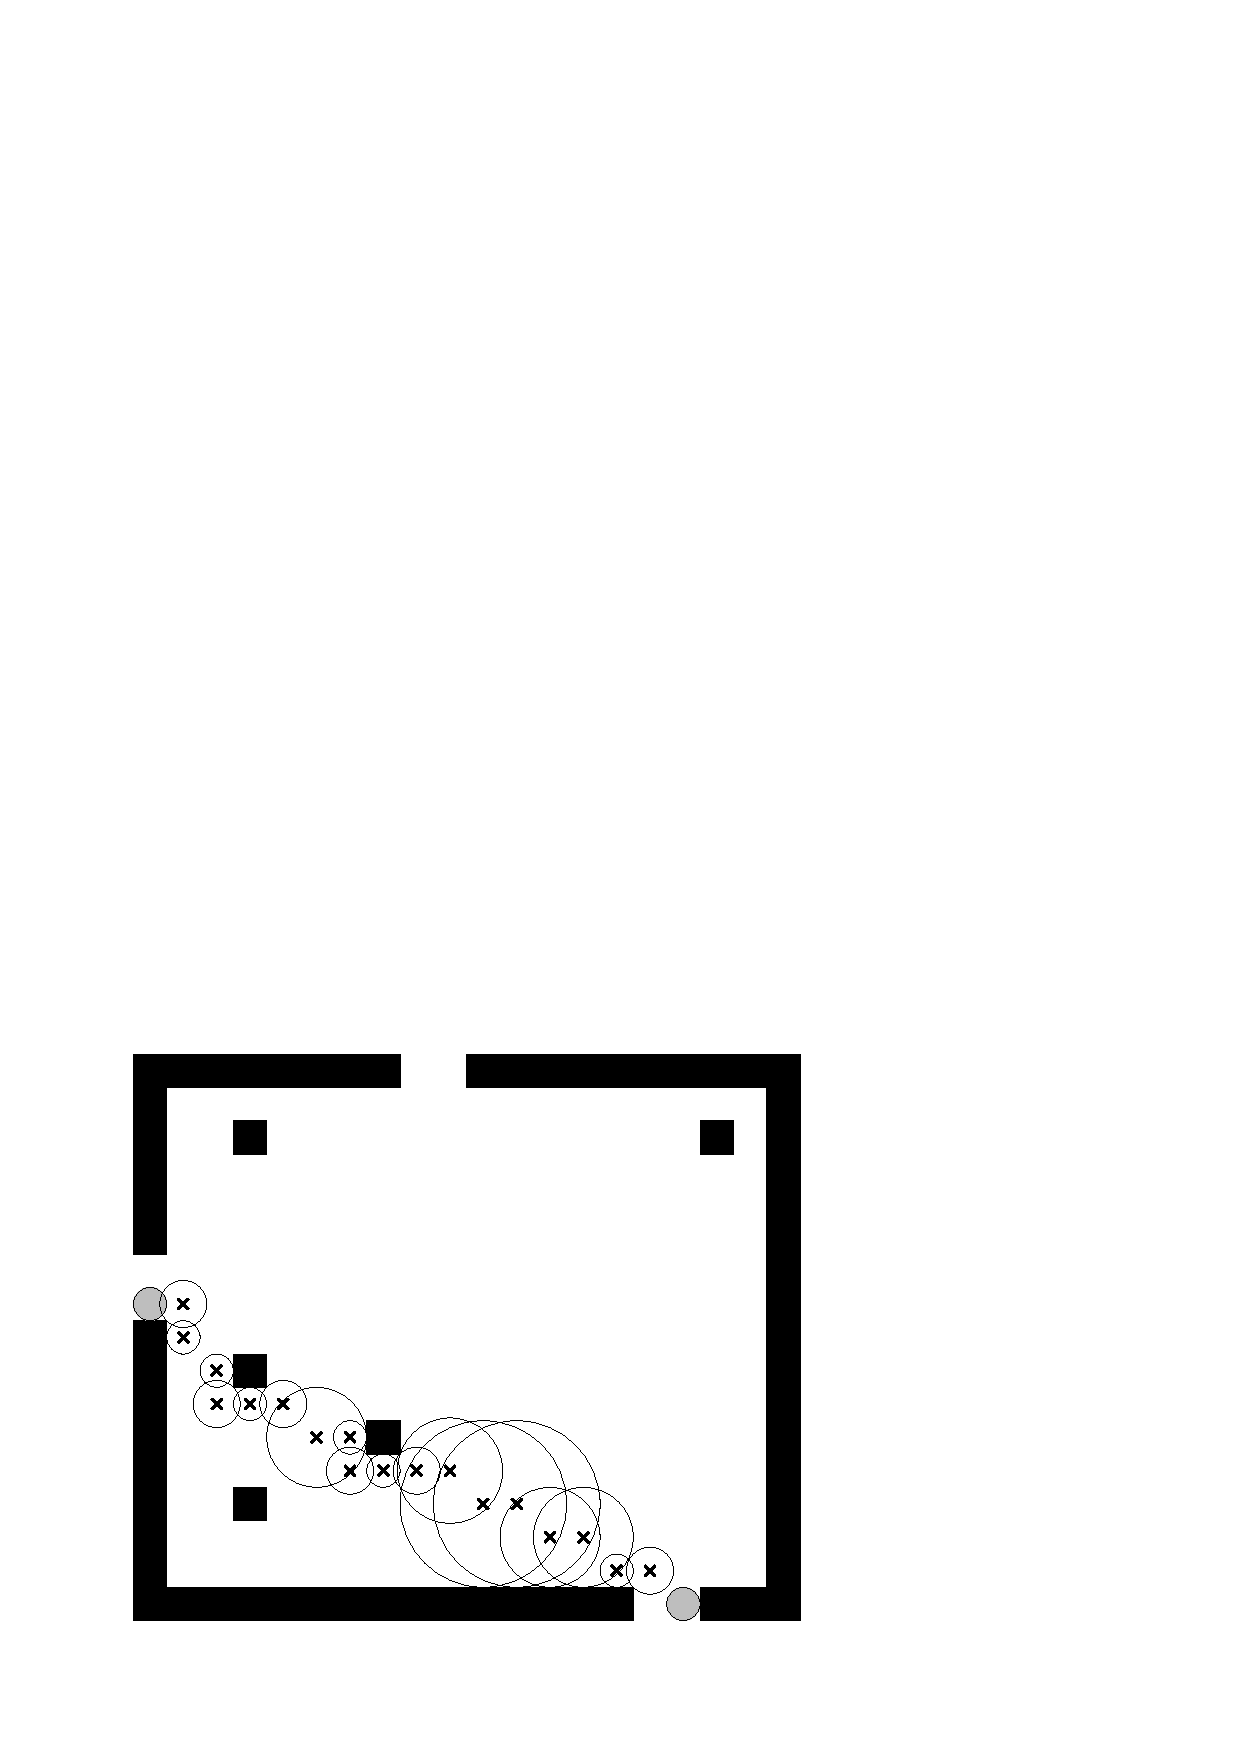
\includegraphics[width=0.30\textwidth]{images/obst_path1.pdf}
\caption{A bad path for groups}
\end{wrapfigure} 
Another problem is what we like to call ``wall hugging slowdown'', which is explained here. The solution for this has not been implemented into the game yet, as current group travel behaviour quickly converges to a line alongside time constraints.
\begin{wrapfigure}{r}{0.30\textwidth}
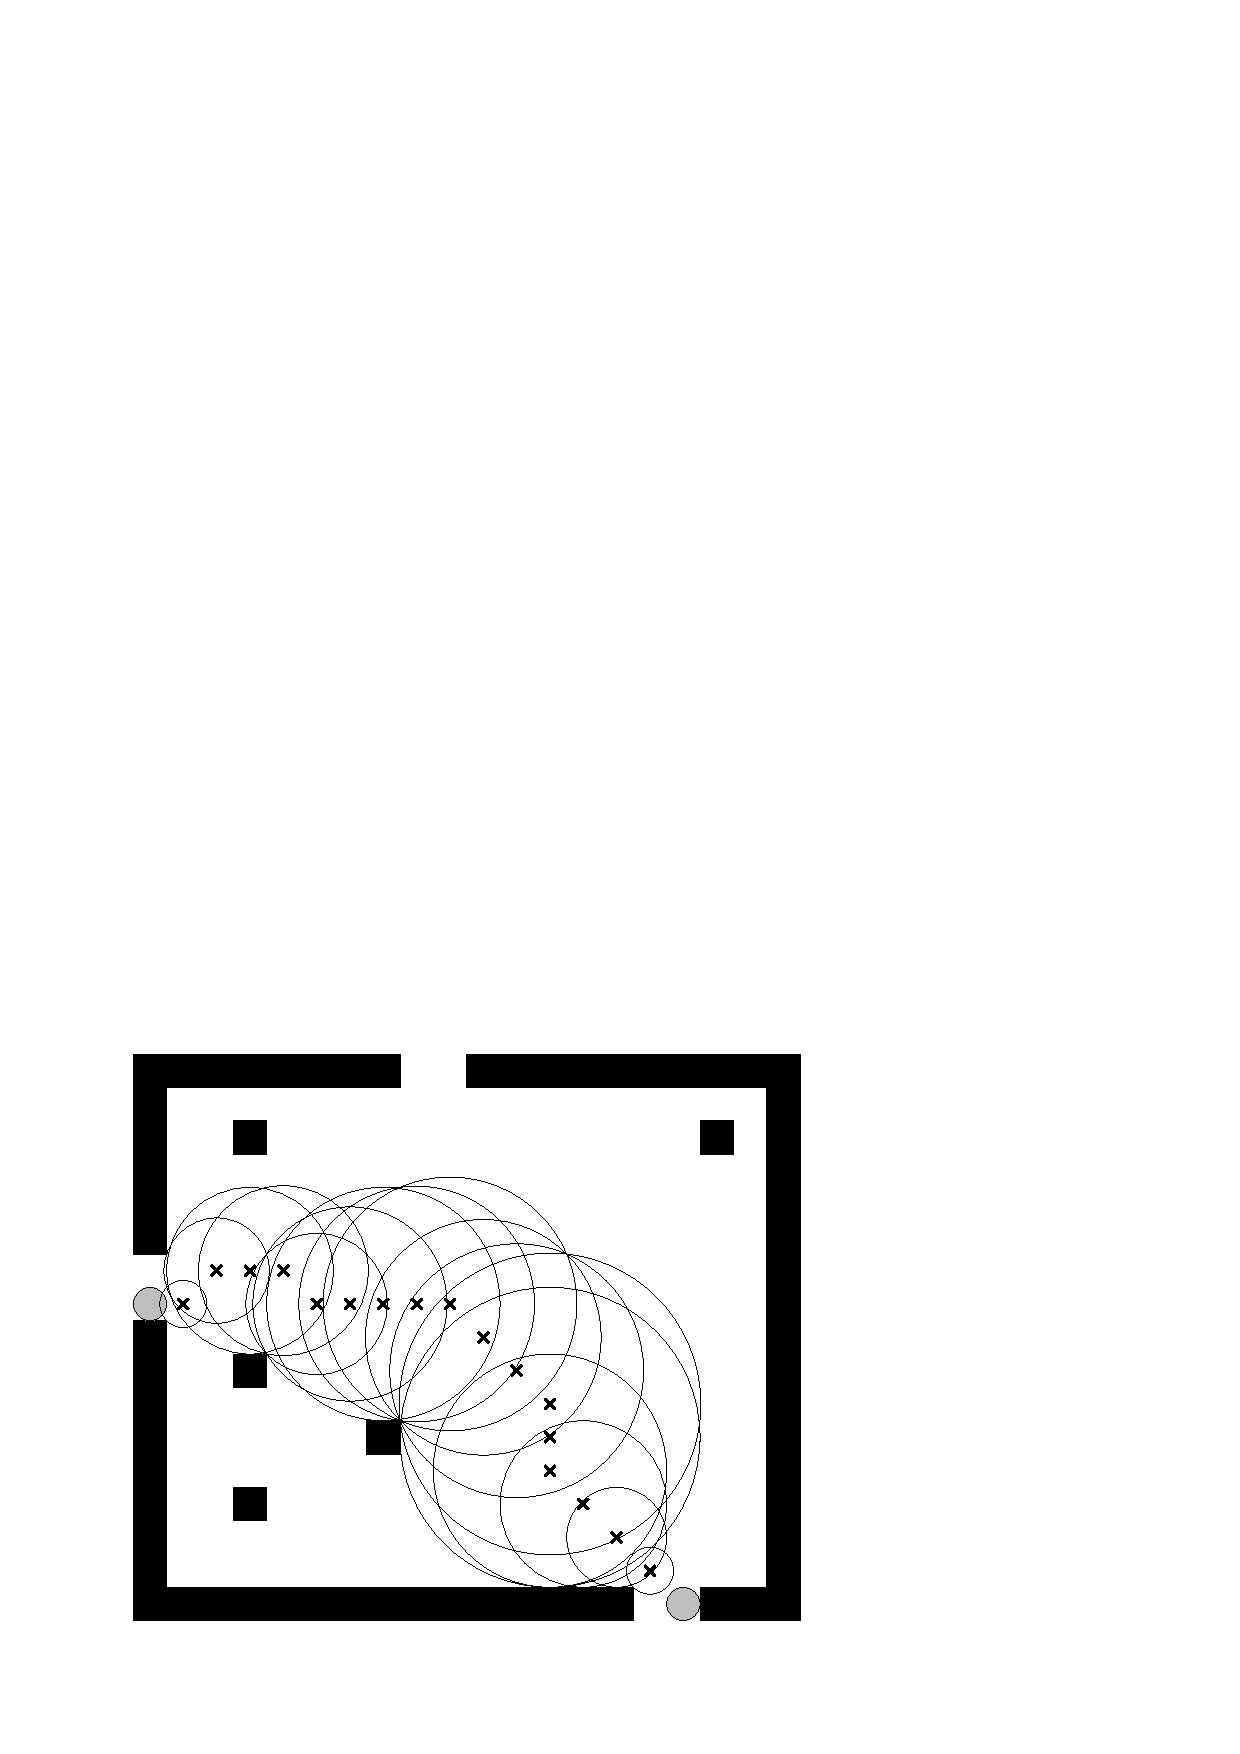
\includegraphics[width=0.30\textwidth]{images/obst_path2.pdf}
\caption{A better path for groups}
\end{wrapfigure} 

A problem that arises with steered movement is that moving along a wall gets slower. The initial slowdown comes from the unit pushing a bit into the wall as it moves along, if the wall is not smooth. A group also cannot take enough space to move in at the wall side. The solution for the scooping problem worsens this, as the radii for cells next to a wall are very small. We solve these problems at once by increasing the weight of cells, depending on their travel radii and the group size. The weight of cells at least the radius of the group away should be uninfluenced. From the group radius up to the cells adjacent to obstacles, the weight should increase at a faster-than-linear rate. We will determine the weight influence based on the following formula:
$$f(r_g, r_t) = \left\{\begin{array}{l l}
					\frac{(r_g - r_t)^p}{s} & \text{if } r_g - r_t > 0\\
					0 & \text{otherwise}
                \end{array}\right.
                $$
Here $r_g$ is the radius of the group, $r_t$ is the travel radius of the cell, and $p$ and $s$ are to be determined by simulation. The radius of the group is actually a function $$r_g(n) = \sqrt{\frac{n * h_u}{\pi}}$$ where $n$ is the number of units and $h_u$ is the surface of the bounding hexagon around a unit.
\begin{wrapfigure}{r}{0.30\textwidth}
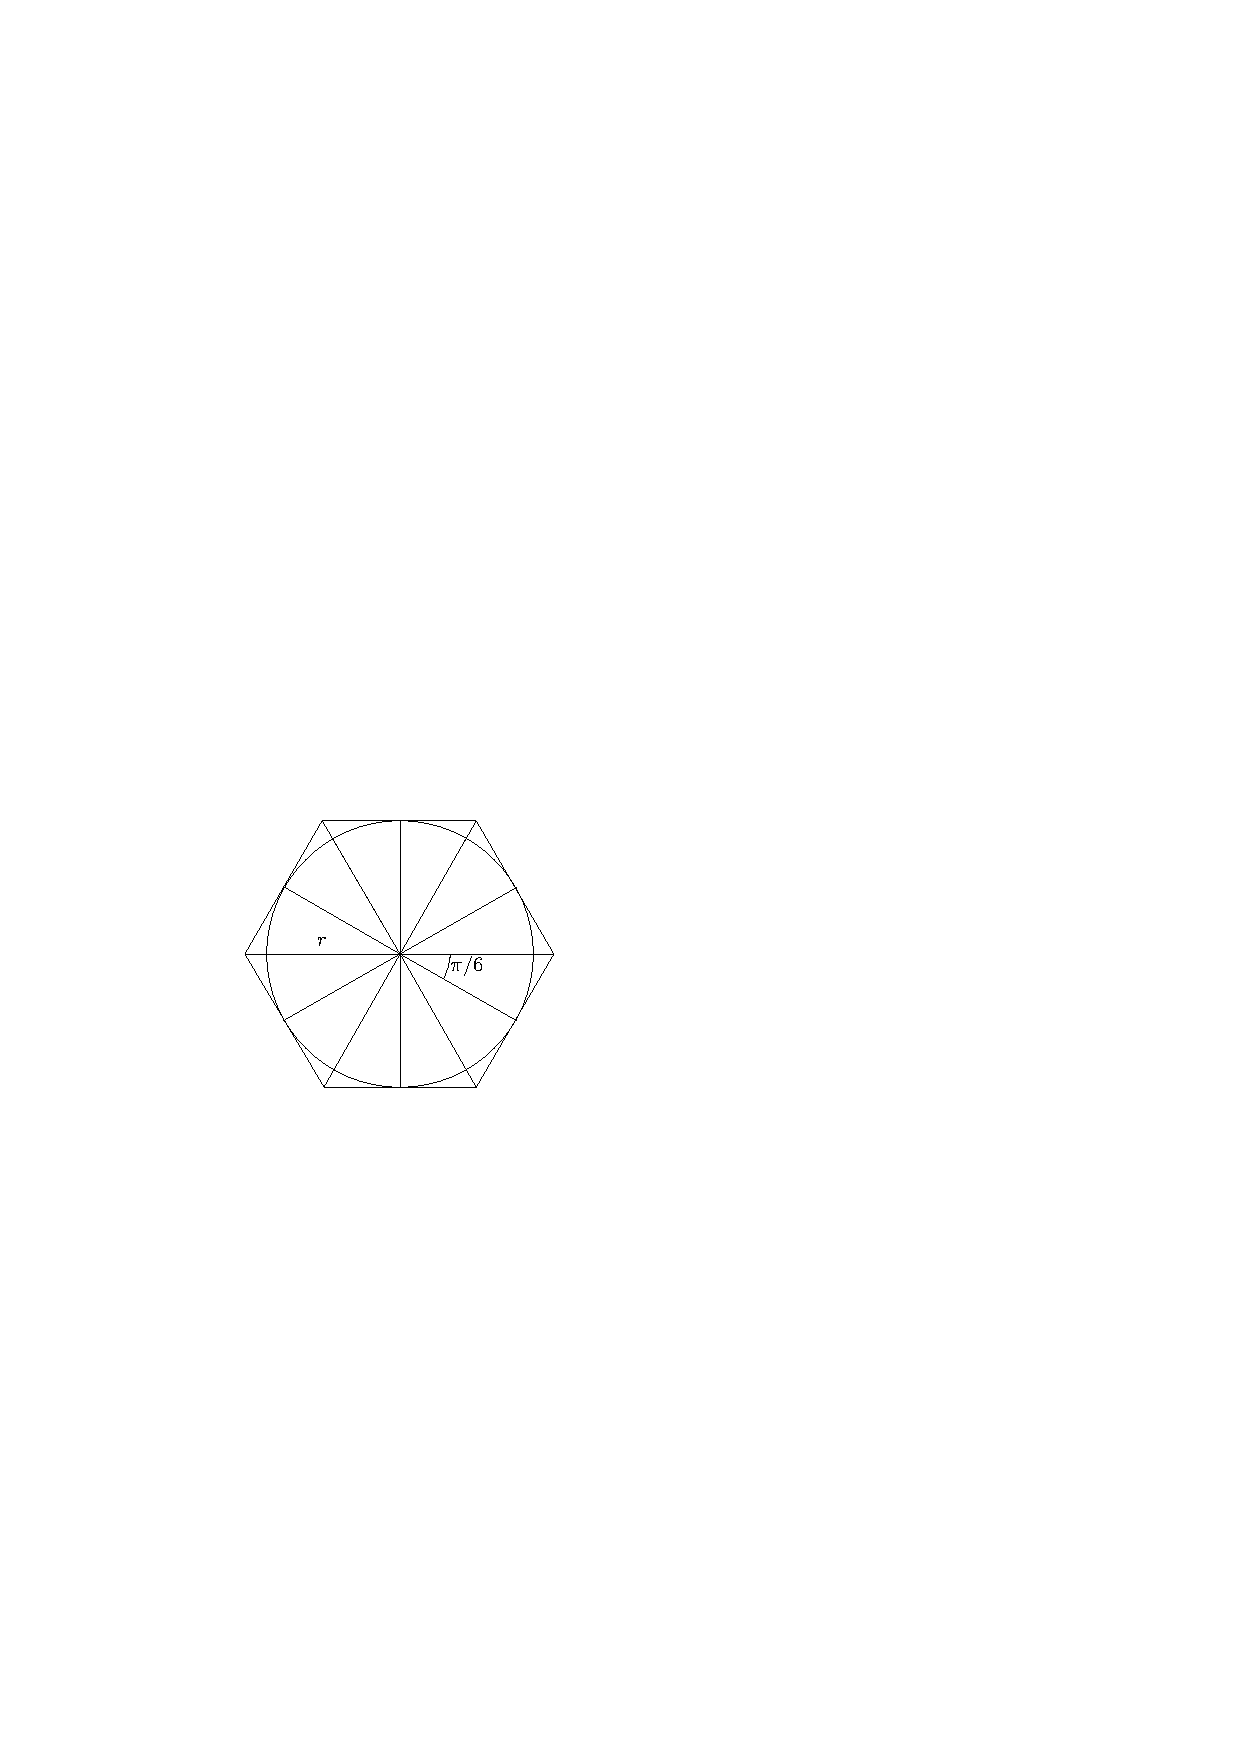
\includegraphics[width=0.30\textwidth]{images/bounding_hexagon.pdf}
\caption{The bounding hexagon}
\end{wrapfigure} 

The surface of this bounding hexagon can be gotten by splitting it up into $12$ right triangles. The angle of the long side and the hypotenuse is $\pi / 6$ for each, and the long side has length $r$, the radius of the circle. The angle gives us that the short side of the triangle is exactly $1/\sqrt{3}$ of the long side. We can combine any two of these triangle surfaces together to make a square surface for easy calculations. This means we have $6$ squares of $r$ long and $r/\sqrt{3}$ wide. The total surface area of the bounding hexagon becomes $h_u = \frac{6r^2}{\sqrt{3}}$. We can throw this back into the group radius formula and simplify further. $$r_g(n) = \sqrt{\frac{n * 6r^2}{\pi * \sqrt{3}}} = r * \sqrt{\frac{n * 6}{\pi * \sqrt{3}}} = r * \sqrt{n*c}$$ Where $c$ simply is a constant: $\frac{6}{\pi * \sqrt{3}}$ 

When moving in urban areas, we may also find that several good paths can be find for small groups, though narrow passages. Large groups will not want to move through these areas when applying this extra weighting. If we can detect these paths during path finding, we could intercept and split the search into multiple paths for smaller groups from there.

\subsubsection{Chunked Maps}
In order to significantly prune the set of things that need to be taken into account for a character to determine its steering force, we used chunked maps. These maps are a coarser grid, similar to the grid used for path finding. In these grids, we keep track of what characters are in what chunk. This way, we can simply take the character and obstacle lists from the nearby chunk and use those lists for calculating steering force.

\subsubsection{Ignoring Parts of the Map}
Since we have to run these steering behaviours constantly on all characters in the map, there might be some performance issues. The group of Vikings the player will typically control is extremely small compared to the map size. Zombies outside of a certain proximity of the Vikings can be simplified in their navigation. This simplification can be done by switching flocking for regular popping from one cell to the next, or by simply letting them stand still.
